% This is samplepaper.tex, a sample chapter demonstrating the
% LLNCS macro package for Springer Computer Science proceedings;
% Version 2.20 of 2017/10/04
%
\documentclass[runningheads]{llncs}
%
\usepackage[utf8]{inputenc}
\usepackage{listings}
\usepackage{xcolor}
\usepackage{graphicx}
\usepackage{tabularx}
\usepackage{hyperref}

\graphicspath{ {./images/} }
\hypersetup{
    colorlinks=true,
    linkcolor=blue,
    filecolor=blue,
    citecolor=blue,
    urlcolor=blue,
    linktocpage=true
}
\setcounter{tocdepth}{2} %show more in the toc

\newcommand{\kw}[1]{\texttt{#1}}
\renewcommand{\contentsname}{table of content}
\usepackage{indentfirst}
\usepackage[english]{babel}

% If you use the hyperref package, please uncomment the following line
% to display URLs in blue roman font according to Springer's eBook style:
\renewcommand\UrlFont{\color{blue}\rmfamily}

%

\title{Infra-estrutura de Testes para Implementações de Referência do Standard ECMAScript}
\subtitle{}

%
\titlerunning{Live Metadata for Test262}
% If the paper title is too long for the running head, you can set
% an abbreviated paper title here
%
\author{Diogo Costa Reis\\ist187526\\
\email{diogo.costa.reis@tecnico.ulisboa.pt}}
%
\authorrunning{Diogo Costa Reis}
% First names are abbreviated in the running head.
% If there are more than two authors, 'et al.' is used.
%
\institute{Instituto Superior Técnico\\
Av. Rovisco Pais, 1\\
1049-001 Lisboa\\
Tel: +351 218 417 000\\
\email{mail@tecnico.ulisboa.pt}}
%


\begin{document}

% a solution to remove title and author from appearing in the table of contents: https://tex.stackexchange.com/a/318220
{\def\addcontentsline#1#2#3{}\maketitle}

%
\begin{abstract}
% TODO

\keywords{ECMAScript \and Specification Language \and Reference Interpreters \and Test262}
\end{abstract}


\newpage

\tableofcontents

\newpage

\section{Introduction}
\label{sec:Introduction}

\section{Goals}
\label{sec:Goals}

\section{Background}
\label{sec:Background}
This chapter provides an overview on the ECMAScript standard, the Test262 that are used to test the correct implementation of the ECMAScript standard, and finally an outline of the new metadata generated.

\subsection{ECMAScript}
\label{subsec:ECMAScript}
% overview da linguagem JS

% paragrafo - porque e' que javascript e' relevante (uma das linguagens mais usadas no momento)
JavaScript (JS) is a programming language mainly used in the development of client side web applications, also being one of the most popular programming languages. According to both GitHub and StakeOverflow statistics, JavaScript finished 2021 as second most active languages on GitHub\footnote{Second most utilized language based GitHub pull requests - https://madnight.github.io/githut/} as well as on StackOverflow.\footnote{Tendencies based on the Tags used - https://insights.stackoverflow.com/trends}



% Boa!
% Existem muitas implementacoes diferentes da linguagem: client-side (browsers), server-side (Node.js), embedded devices (Jerryscript) -> Estas implementacoes têm de estar de acordo no comportamento observavel -> é particularmente importante na Web -> senao temos sites que em ...
% -----------------------
% overview do standard -> descrita num standard
% Porque é muito importante que as várias implementacoes da linguagem coincidam -> o JavaScript está especificado num documento semi-formal que ...
% Falar sobre o standard
%   - o standard está como um interpretador de JavaScript em
%     pseudo-codigo - descreve detalhadamente os passos que
%    um interpretador de JS tem de executar ao avaliar qualquer
%    statement da linguagem
% Falar sobre o comité -  quem controla a evolucao do ECMAScript
ECMAScript standard\cite{ECMAScriptStandard} is the official document, written in the English language, in which the JavaScript language is defined. This document is in constant evolution, being updated by the ECMA Technical Committee 39 (TC39), which is responsible for maintaining the standard. The standard is currently in its twelfth version.
%
The standard specifies the \texttt{JavaScript} language, to ensure its multiple compilers and interpreters implementations are coherent. Some of the \texttt{JavaScript} compilers are the Hop~\cite{Hop} and the JSC~\cite{JSC} compilers, the most popular interpreters are Node.js~\cite{Node.js} and SpiderMonkey~\cite{SpiderMonkey}. These are only four implementations among many others, which come along with the many use cases that \texttt{JavaScript} has.
%
\texttt{JavaScript} is mostly used in the web context, both client-side within browsers and server-side, but also in embedded devices. Since \texttt{JavaScript} is used in so many scenarios and across so many different contexts, it is highly important that ECMAScript standard is defined in great detail to ensure consistency. Browsers, for example, need to run \texttt{JavaScript} implementations that coincide so that websites are correctly rendered and exhibit the same behavior. In order to achieve coherent implementations, the standard defines the types, values, objects, properties, syntax, and semantics of \texttt{JavaScript} that must be the same in every \texttt{JavaScript} compiler and interpreter, while allowing \texttt{JavaScript} implementations to define additional types, values, object, properties, and functions.




% Good, more detail if there is time
% Estrutura do standard
The \texttt{JavaScript} language can be divided into three major components, those being expressions and commands, built-in libraries, and finally internal functions.
%
\begin{itemize}
\item Expressions and commands describe the behavior of static constructions, detailing the semantics of the diverse expressions (e.g., assignment expressions, built-in operators, etc.), commands (e.g., loop commands, conditions command, etc.), and built-in types (Undefined, Null, Boolean, Number, String and Object).
%
\item The internal functions of the language are used to define the semantics for both expressions and commands, as well as the built-in libraries. Internal functions are not exposed beyond the internal context of the language. In other words, no JavaScript program uses internal functions directly.
%
\item Finally, built-in libraries encompass all the internal objects available when a JavaScript program is executed. Internal objects expose many functions implemented by the language itself, including functions to manipulate numbers, text, arrays, objects, amongst other things.
\end{itemize}


% MetaParagrafo tres tipos
\colorbox{orange}{The remaining} subsection provides a description of the three types of artifact described in the standard.
% QUESTION ainda nao foi lido pelo prof

% Expressions and statements
% Exemplo do standard  e explicacao (if)
\paragraph{Semantics of IF statement}
Figure \ref{fig:If-Else Statement} shows a snippet of the ECMAScript standard description of the \texttt{IF} command. In order to evaluate \texttt{IF} commands with the shape:

\begin{center}
\texttt{if (Expression) Statement1 else Statement2}
\end{center}

\noindent the language begins by evaluating the \texttt{Expression} storing the result in the variable \texttt{exprRef} (step 1). The previous step will be used as Boolean, therefore, the result of the previous step will be converted to a Boolean using the internal functions \texttt{ToBoolean} and \texttt{GetValue}, and having the result stored in the variable \texttt{exprValue} (step 2).A different \texttt{Statement} will be followed depending on \texttt{exprValue}. If \texttt{exprValue} has the value \texttt{true} the variable \texttt{stmtCompletion} will have the evaluation of the first \texttt{Statement} (step 3). Otherwise, the variable \texttt{stmtCompletion} will store the result of evaluating the second \texttt{Statement} (step 4). Finally, a \texttt{Completion} will be returned, if the \texttt{stmtCompletion} has non empty value then it will be returned, however, when the value is empty it will be replaced with undefined (step 5).

\begin{figure}[ht]
    \centering
    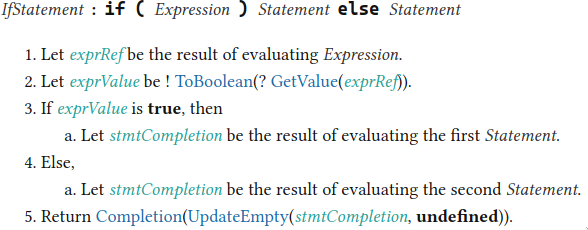
\includegraphics[width=0.8\textwidth]{images/if_statement.png}
    \caption{ECMAScript definition of an if-else statement}
    \label{fig:If-Else Statement}
\end{figure}

% arrays são objetos como os outros
% arrys tem propriedades especiais
% example of Array.pop
% Built-ins (Array.pop)
% printscreen do standard e explicacao
\paragraph{Semantics of the Pop function}
The Array built-in is an object as any other in JavaScript. The main difference is in its properties. Array Objects have a property \texttt{length} that contains the size of the array, as well as a property for each element of the array (from zero to \texttt{length} minus 1).

Figure \ref{fig:Array_pop_example} shows a simplified version of an array performing the pop function, where \texttt{(a)} and \texttt{(b)} are the before and after respectively.
Before preforming \texttt{pop} \texttt{(a)}, the array has three  properties \texttt{length}, \texttt{0}, and \texttt{1}. Property \texttt{length} represents the size of the array that has value \texttt{2}, while the properties \texttt{0} and \texttt{1} store the first (\texttt{banana}) and second (\texttt{kiwi}) elements of the array respectively.
After \texttt{pop} is preformed \texttt{(b)}, the last element is of the array is removed (highlighted in red at \texttt{(a)}) and the \texttt{length} property (highlighted in green) is decremented by one since the size of the array changes to one.

% TODO change length with quotation marks
\begin{figure}[ht]
    \centering
    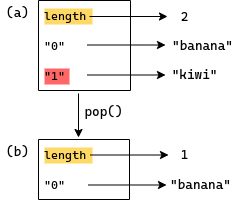
\includegraphics[width=0.4\textwidth]{images/array_pop_example.png}
    \caption{Example Array.pop}
    \label{fig:Array_pop_example}
\end{figure}
Figure \ref{fig:Array_pop} shows a snippet of the ECMAScript standard description of the pop function in the Array Built-in. To begin with, the array will be converted to and Object using the \texttt{ToObject} function, and stored in the \texttt{O} variable (step 1).
Afterwards, the array length of the previously calculated variable will be calculated with the \texttt{LengthOfArrayLike} internal function, and storing the result in the \texttt{len} variable (step 2).
At this point there are to ways to proceed depending on the value of \texttt{len}. If the value is zero, the Array is empty, then the property \texttt{length} of \texttt{O} is set to zero and \texttt{undefined} is returned (step 3).
Otherwise, when \texttt{len} is different from zero, meaning that the Array is not empty, the Array's last element will be removed (described in Figure \ref{fig:Array_pop_example}) and returned (step 4).
To begin with, the language will assert that \texttt{len} is positive (step 4.a).
Afterwards, the \texttt{newLen} variable will store the value of \texttt{len} decremented by 1 (step 4.b).
The variable \texttt{index} will store the variable calculated in the previous step represented as a String converted with the \texttt{toString} function (step 4.c).
Then, stores the value of the \texttt{O} variable at the property corresponding to \texttt{index} in the \texttt{element} variable using the \texttt{Get} function (step 4.d).
Subsequently, deletes the previously mentioned property of the \texttt{O} variable with the \texttt{DeletePropertyOrThrow} function (step 4.e).
In addition, sets the \texttt{length} property of the \texttt{O} variable  to the \texttt{newLen} using the \texttt{Set} function (step 4.f).
Finally, returning the value of the variable \texttt{element} (step 4.g).

\begin{figure}[ht]
    \centering
    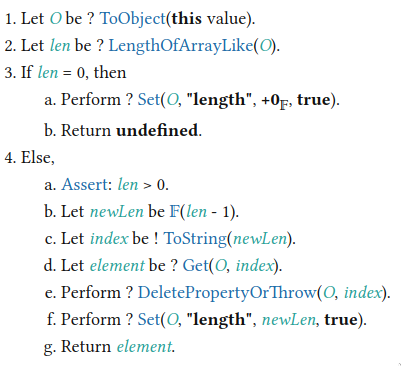
\includegraphics[width=0.6\textwidth]{images/array_pop.png}
    \caption{ECMAScript definition of Array.pop}
    \label{fig:Array_pop}
\end{figure}



% Internal Functions (LenghtOfArrayLike)
% printscreen do standard e explicacao
\paragraph*{LengthOfArrayLike internal function}
Figure \ref{fig:LengthOfArrayLike} shows a snippet of the ECMAScript standard description of the \texttt{LengthOfArrayLike} internal function, that evaluates the function:

\begin{center}
\texttt{LengthOfArrayLike (obj)}
\end{center}

\noindent The language starts by asserting that \texttt{obj} is an \texttt{Object} (step 1). Afterwards, gets the value of the property \texttt{length} from \texttt{obj} using the function \texttt{Get}. Then, converts the previously mentioned value to an Integer that represents the length with the \texttt{ToLength} function, and finally returns said Integer (step 2).

\begin{figure}[ht]
    \centering
    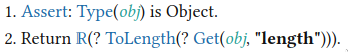
\includegraphics[width=0.5\textwidth]{images/length_array_like.png}
    \caption{ECMAScript definition of the LengthOfArrayLike}
    \label{fig:LengthOfArrayLike}
\end{figure}




\subsection{Test262}
\label{subsec:Test262}


% paragrafo - JS tem muitas particularidades que dificultam o desemvolvimento e testagem  -> É muito dificil desenvolver
% novas implemenentacoes da linguagem
% Existe uma bateria de testes que testa as implementacoes da
% linguagem contra o standard
% Esta bateria de testes é dificil de manter
% Porque? - muitos testes, muitas features, em geral ha retrocompatibilidade mas ha um pequeno numero de casos onde a retrocompatibilidade nao se verifica -> os testes de ser modificados
Implementing a \texttt{JavaScript} engine is particularly difficult since it involves dealing with the many corner cases that exist in the language. To test that corner cases are correctly dealt with there is \texttt{Test262}\cite{Test262}, the ECMAScript standard test battery. Although, \texttt{Test262} is vital to the \texttt{JavaScript} engines, it is very hard to maintain due it's complexity, the total number of tests is around \colorbox{orange}{39837} divided into \colorbox{orange}{87} subfolders, each correspond to roughly one section of the standard. \texttt{Test262} complexity grows with changes to the standard since in most cases backward compatible is maintained except for a few select cases. 
% 87 subfolders on built-ins + language
% QUESTION round number? (40000)
% QUESTION 105 subfolders if add intl402 (which also has files that were ignore)



% Implementacoes parciais da linguagem 
% Na acadamia é normal desenvolverem-se implementacoes parciais da linguagem: não suportam a ultima versao, não suportam todos os objectos built-in, não suportam todas
% Pergunta: Quais é que são os testes apropriados?
% Normal: Respostas ad-hoc -> sem justificação rigorosa -> basicamente cada paper selecciona os testes que lhe da jeito
Due to the ECMAScript standard being so extensive most implementations are only partial, especially implementations and analysis developed in academic contexts. In order to test partial implementations, one must be able to obtain the applicable set of tests from all the tests contained in Test262. Selecting the applicable tests is not a trivial matter because there are too many tests and too many features. The current methodology is that each development team manually selects the tests that are applicable to their corresponding implementation. This raises the problem that there is not standard and precise way of picking the all the right tests from the almost 40000 tests in \texttt{Test262}, making the possibility of human error when selecting the applicable tests likely.


% gosto
%% Formato dos testes
% frontmatter, code
% exemplo
Figure \ref{fig:Test262_example} shows a test from \texttt{Test262}. Every test of \texttt{Test262} has 3 parts: first is the copyright section represented with the comment \texttt{//} (lines 1 and 2), second is the \texttt{Frontmatter} section between \texttt{/*---} and \texttt{---*/} with some metadata about the test (lines 4 to 7), and finally is the \texttt{Body} section with the code of the test (lines 9 to 13). The copyright section has information about the owner and license of the test. The \texttt{Frontmatter} section has the test id (15.4.5-1) and a description of the test. Finally, the \texttt{Body}'s code tests the correct implementation of the standard.

\begin{figure}[ht]
    \centering
    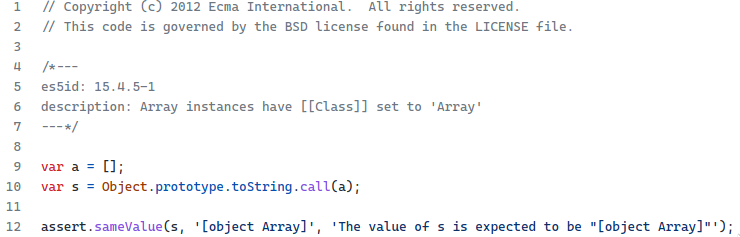
\includegraphics[width=1.0\textwidth]{images/test262_array_test.png}
    \caption{Test262 es5id: 15.4.5-1}
    \label{fig:Test262_example}
\end{figure}



%% metadados ja incluidos
%% referir outra vez o exemplo
% - metadados oficialmente incluídos nos testes
%   - que metadados é que os testes contém actualmente
The \texttt{Frontmatter} has keywords to hold metadata of the test. These keywords are associated with specific elements of metadata concerning the test. Bellow is the list of possible keywords and their meaning:

\begin{itemize}
\item \texttt{description} - contains a short description about what will be tested;
%
\item \texttt{esid} - contains the hash identifier of the ECMAScript portion associated with the feature that will be tested (the identifier references the most recent version of ECMAScript when the test is created);
%
\item \texttt{info} - contains a deeper explanation of the test behavior, frequently includes a direct citation of the standard;
%
\item \texttt{negative} - indicates that the test throws an error; associated to the keyword will be the type of error the test is supposed to be thrown (e.g. \texttt{TypeError}, \texttt{ReferenceError}) as well as the phase in which the error is expected to be thrown (e.g. \texttt{parse} vs \texttt{resolution} vs \texttt{runtime});
%
\item \texttt{includes} - contains the list of \texttt{harness} files that should be included in the execution of the tests (\texttt{Test262} makes use of a large number of auxiliary function defined in a dedicated library referred to as the \texttt{Test262} \texttt{harness} described later in this section);
%
\item \texttt{author} - contains the identification of the author of the test;
%
\item \texttt{flags} - contains a list of booleans for each test property, the properties being: (1) \texttt{onlyStrict}, the test is only executed in strict mode; (2) noStrict, the test will only be executed in mode \emph{sloppy}; (3) \texttt{module}, the test must be integrated as a \texttt{JavaScript} module; (4) \texttt{raw}, executes the test without any modification, which implies running as \texttt{noStrict}; (5) \texttt{async}, the test is contains asynchronous functions; (6) \texttt{generated}, the test generates the files specified by the property; (7) \texttt{CanBlockIsFalse} and (8) \texttt{CanBlockIsTrue}, the test will run if the property \texttt{CanBlock} of the \colorbox{orange}{\texttt{Agent Record}} executing it is false and true respectively; (9) \texttt{non-deterministic}, indicates that the semantics used in the test are intentionally under-specified and therefore the test passing or failing should not be regarded as an indication of reliability or conformance;
% QUESTION clarificar se e' necessario citar o que e' 'Agent Record' uma vez que nao vou explicar
%
%
\item \texttt{features} - contains a list of features that are used in the test;
%
\item \texttt{es5id} and \texttt{es6id} - indicates that the feature being tested belongs to ECMAScript 5 and 6 respectively and contains the hash identifier of the section of the standard it belongs to; these keywords have been deprecated and substituted by esid.
\end{itemize}


% Varias observacoes: 
%  - A metada esta muitas vezes INCOMPLETA e algumas vezes incorrecta 
%  - é preciso calcular a metadata certa
As Figure 5 illustrates, it is often the case that the metadata of a test is incomplete. Some tests also have the wrong metadata. As part of this thesis, we plan to process all the tests to check and correct their corresponding metadata as well as completing the metadata that is \colorbox{orange}{missing.}

%% QUESTION juntar os paragrafos?

%% metadados que achamos relevantes e nao estao incluidos
%% ...
\colorbox{orange}{The example} in Figure \ref{fig:Test262_example} has 2 keywords, description and the deprecated es5id. Besides the obvious upgrade from \texttt{es5id} to \texttt{esid} it would be useful to have \texttt{includes} with the \texttt{harness} files needed to execute the test. The \texttt{harness} information is very useful since it makes it easy to identify the part of the \texttt{harness} needed to run that test, opening the door for loading only part of the \texttt{harness} instead of the whole \texttt{harness} which is the current approach.



% - quais são os metadados que nós achamos serem relevantes e que estão em falta
\paragraph{New Metadata}
In order to have a more complete \texttt{Frontmatter} we suggest adding the following information:

\begin{itemize}
    \item \texttt{syntactic construct} - list of all syntactic constructions used in the test;
    \item \texttt{version} - the ECMAScript version of the standard in which the feature being tested was introduced;
    \item \texttt{built-ins} - list of all the built-ins used in the test.
    \item \colorbox{orange}{\texttt{harness-functions}} - list of all the harness functions used to asses the test's results.
\end{itemize}
% QUESTION posso adicionar isto? acho que era suposto fazer parte da minha tese; se calhar nao faz sentido, mas sim ter a informacao do includes segundo o standar (com o nome dos ficheiros da harness necessarios para o test)

This metadata provides helpful information to solve the problem mentioned before, selecting the applicable tests for partial implementations, by allowing developers to filter tests by \texttt{builtin}, \texttt{static construct} and \texttt{version} of the \texttt{ECMAScript} standard. This would provide consistency and standardization to the selection of applicable tests to a partial implementation of the standard. As for the \texttt{harness-functions}, it provides the information of about the functions of \texttt{harness} that are used in the test, that is relevant because only a small part of the \texttt{harness} is need in each test even though the \colorbox{orange}{whole library is loaded}.
% QUESTION suponho que o maior problema seja que todos testes da harness sejam corridos e nao o facto de toda a biblioteca seja carregada





\subsection{An Infrastructure for testing reference implementations of the ECMAScript standard}
\label{subsec:An Infrastructure for testing reference implementations of the ECMAScript standard}

% Resumo da tese do Miguel 
This thesis continues the work done in the master thesis of Miguel Trigo titled \emph{Infra-estrutura de Testes para Implementações de Referência do Standard ECMAScript}. In Miguel Trigo's master thesis, he \colorbox{orange}{processed} all Test262 tests and checked their metadata,  correcting some errors that \colorbox{orange}{were} found and complementing some metadata that is missing in the \texttt{Frontmatter}. The author also added new metadata that out of the scope of the \texttt{Frontmatter}, added statistical data about the tests, and made all the previously mentioned data available in a \texttt{MongoDB} database.
% QUESTION da' a sensacao que o miguel fez tudo a mao? devia mencionar que ele automou o processo de gerar metadata?
% QUESTION past tense?


% - Corrigir a metadata dos testes incorrectos e calcular metadata adicional ????
% - construir uma base de dados com a metadata dos varios testes em formato JSON 
Miguel Trigo processed the test in Figure \ref{fig:Test262_example} and generated the metadata in Figure \ref{fig:json_metadata}. The \texttt{Frontmatter} in the test has the \texttt{es5id} and \texttt{description}, in the generated metadata they are represented for the \texttt{name} and \texttt{value} pairs \texttt{esid} and \texttt{description} respectively \colorbox{orange}{(updating the deprecated es5id)}.
% QUESTION conta como correcao? eu devo arranjar um exemplo de uma correcao que ele fez? ou so' mensionar?
%
%
The following \texttt{names} were added by Miguel Trigo:

\begin{itemize}
    \item \texttt{path} - stores the path to the test within \texttt{Test262};
    \item \texttt{version} - stores the version of the \texttt{ECMAScript} standard that the test corresponds to;
    \item \texttt{built-ins} - stores a subpart of the \texttt{path};
    \item \texttt{Array} - stores the subpart of the \texttt{path} that follows \texttt{built-ins};
    \item \texttt{syntactic\_construct} - stores an array with all the syntactic constructions used in the test;
    \item \texttt{builtIns} - stores an array with all the builtins used in the test;
    \item \texttt{asserts} - stores the number of times the \texttt{assert} library is used in the test;
    \item \texttt{error} - \colorbox{orange}{TODO Nao sei o que representa};
    \item \texttt{esprima} - stores whether or not the test is supported by \texttt{Esprima}\cite{Esprima} (\texttt{Esprima} is an standard-compliant \texttt{ECMAScript} parser that is also developed in \texttt{ECMAScript});
    \item \texttt{lines} - stores the number of lines of code written in the test, ignoring the empty lines and comments (in this example the \texttt{value} is 3 because lines 12 and 13 in Figure \ref{fig:Test262_example} are one single line in the actual test in \texttt{Test262} that was split in the example to make the image more legible).
\end{itemize}

% Exemplo
\begin{figure}[ht]
    \centering
    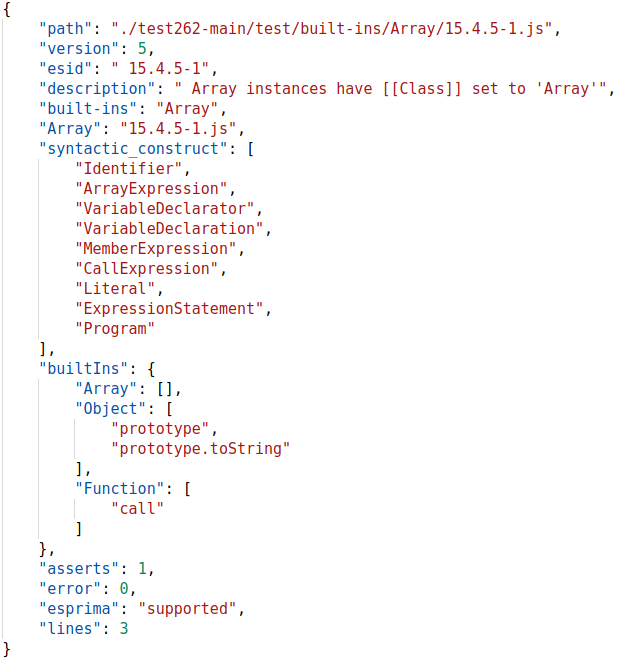
\includegraphics[width=0.9\textwidth]{images/json_metadata.png}
    \caption{Metadata generated for test esid: 15.4.5-1.js}
    \label{fig:json_metadata}
\end{figure}

The metadata can be separated into four parts. Firstly, the \texttt{Frontmatter} part, \texttt{description} and \texttt{esid}, that stores information related to the \texttt{Frontmatter} of the test. Secondly, the path part comprised of \texttt{path}, \texttt{built-ins}, and \texttt{Array}, that contains the information related to the path of the test inside the \texttt{Test262}. Thirdly, the statistical part formed by \texttt{asserts}, \texttt{error}, \texttt{esprima}, and \texttt{lines}, that provides statistics on the code of the test and the metadata generation process.
%
% - Metadata adicional calculada para cada teste:
Finally, the new metadata part which consists of \texttt{version}, \texttt{syntactic\_construct}, and \texttt{builtIns}, the new metadata is relevant information about the tests that should be added to the \texttt{Frontmatter}.



% Para cada um dos tipos de metadata 
In the remaining of the subsection is concerned with how the new metadata, namely \texttt{syntactic\_construct}, \texttt{builtIn}, and \texttt{version}.


% - how syntactic cosntruct is calculated 
\paragraph{Calculation of syntactic\_Construct metadata}
The \texttt{syntactic\_construct} metadata is calculated with the help of \texttt{Esprima}, which allows the analysis of the \colorbox{orange}{syntactic tree} of the test. The tree analysis of the test is represented in a JSON format and the \texttt{syntactic\_constructs} are the \texttt{values} corresponding to the \texttt{names} \emph{type} of every element of the tree. This way, to get all the \texttt{syntactic\_construct} is only a matter of traversing the tree and adding any new one found. The main problem being that \texttt{Esprima} only supports till version 7 of the \texttt{ECMAScript} standard, and also the \texttt{negative} tests that \texttt{Esprima} does not support.
% QUESTION imagem do JSON retornado pelo esprima?
\begin{figure}[ht]
    \centering
    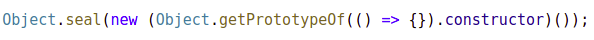
\includegraphics[width=0.9\textwidth]{images/test_syntactic_tree.png}
    \caption{Example test}
    \label{fig:test_syntactic_tree}
\end{figure}
\begin{figure}[ht]
    \centering
    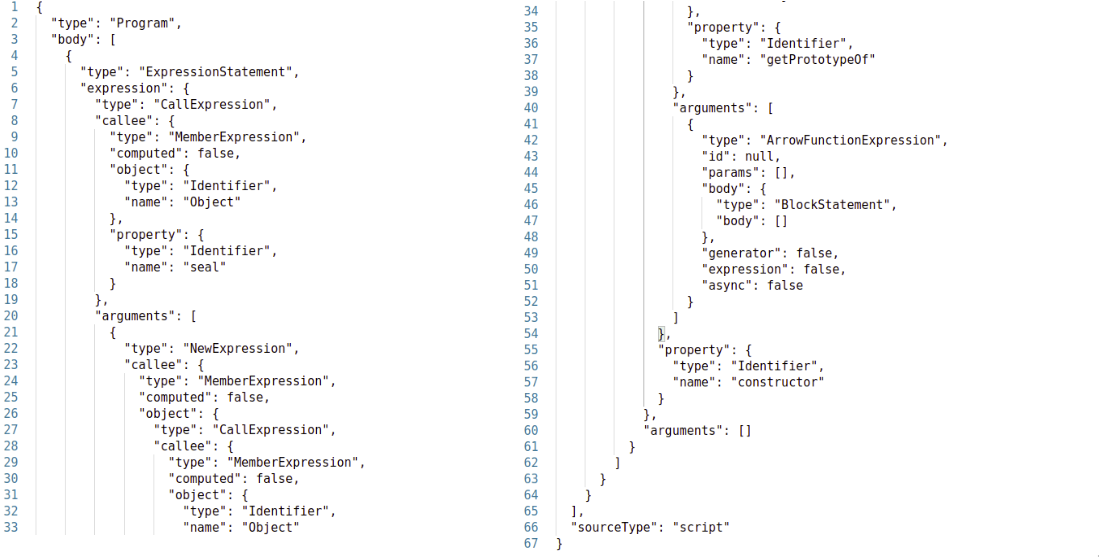
\includegraphics[width=1\textwidth]{images/JSON_syntactic_tree.png}
    \caption{syntactic tree of the example test in Figure \ref{fig:test_syntactic_tree}}
    \label{fig:JSON_syntactic_tree}
\end{figure}

% - how built-ins is calculated
\paragraph{Calculation of built-ins metadata}
The \texttt{built-ins} are calculated with two separate methods. The first method makes use of syntactic tree generated from \texttt{Esprima}, to find key \texttt{static\_constructs} to identify the \texttt{built-ins} being used. While the second method goes through the code of a test and finds all the functions and associates them with their \texttt{built-ins}, as well as the finding \texttt{built-ins} being used directly. In both methods, after all the \texttt{built-ins} of a test are identified, the \texttt{built-in} that corresponds to the most recent version of the \texttt{ECMAScript} standard identifies the version of that test. 


% - how version is calculated 
\paragraph{Calculation of Version metadata}
The \texttt{version} metadata is calculated by identifying the element, \texttt{built-in}, \texttt{syntactic\_construct} or change in behavior of functions that is part of the newest version of the \texttt{ECMAScript} standard. The version is calculated using 3 different approaches dynamic, static, and mixed.
%
The dynamic approach is based on the waterfall model, running the tests against an implementation of the standard. if the test passes then the test is associated with that version of the standard, otherwise the test will be run against the next version of the implementation of the standard.
%
The static approach uses the syntactic tree generated with \texttt{Esprima}. From the analysis of the syntactic tree all the objects, functions, properties, operators, variables, and syntactical constructions present in the test are found, then searches for the oldest version that contains all of them.
%
The mixed approach is calculated using the dynamic and static approaches. The mixed approach consists of running the results of the dynamic approach of each version and verifying that is does not use features introduced in a posterior version. The dynamic approach makes use of \texttt{SpyderMonkey} and \texttt{Node.js} implementations of the standard. 

\begin{figure}[ht]
    \centering
    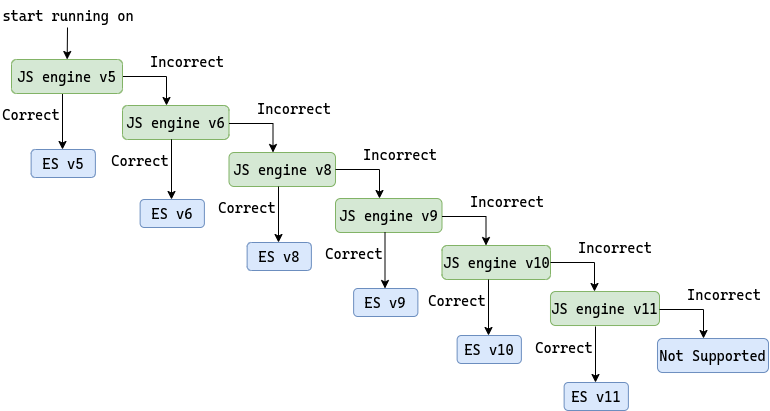
\includegraphics[width=1\textwidth]{images/waterfall_model.png}
    \caption{waterfall model of the dynamic approach}
    \label{fig:waterfall_model}
\end{figure}



\section{Related Work}
\label{sec:Related Work}



\section{Design and Methodology}
\label{sec:Design and Methodology}



%  grandes objectivos 
This thesis is a continuation of Miguel Tringo's master thesis, aiming to complete the calculation of the \texttt{Frontmatter} metadata especially the \colorbox{orange}{metadata about the \texttt{harness}}, also aims to improve the generated metadata. Another aim of this thesis is to create a website for visualizing the metadata generated. \colorbox{orange}{Finally,} we aim to build a platform that allows users to submit the markdown generated from executing the \texttt{Test262} and compare different runs.
% QUESTION campo features? (restantes talvez possam ser ignorados author, negative, flags, info and description)
% QUESTION incluir?



% - processamento completo da metadata oficial 
% -> o processamento do miguel esta incompleto -> nao incluir informacao informacao sobre -> ... 
% [pode criticar como entender]
Miguel Trigo's thesis metadata is incomplete in various ways, tests with unknown \texttt{version} around 9000, tests without \texttt{built-ins} around 17000, and tests without \texttt{syntactic\_construct} around 13000 \colorbox{orange}{tests without esid around 600}.
% QUESTION sao tests da versao seginte de ECMA que ainda nao tem seccao na versao actual?
%
The metadata from the thesis could be improved in way the data is arranged, for example, the subfolders of the path to the test are spread into the JSON Object of the test. The subfolders information being put into an array of ordered subfolders would increase the readability.



% - calculo mais preciso da nova metadata proposta
% - o calculo da versao pode ser melhorado de varias maneiras
This thesis plans to improve the \texttt{version} metadata generation in two dimensions precision and efficiency.
% - Precisao 
% - usar mais engines
For the precision, with more \texttt{JavaScript} engines being used, there would be more certainty when determining the version.
% - Eficiencia 
% - paralelizar os engines 
As for the efficiency, it would be possible to parallelize the waterfall model of the dynamic approach running multiple tests at the same time. It is also possible to use \texttt{git diff} to identify the tests that were added or changed since the last time the dynamic approach was executed, \colorbox{orange}{ only needing to execute} the dynamic approach on the differences.
% QUESTION e' problema se fizerem update noutro lado que afeta o teste indiretamente?



% - Sistema de visualisacao da metadata 
The website for visualizing the metadata aims to make access to the metadata and filtering it easily accessible. The website is planned to allow the search 



% printscreens do site 
\begin{figure}[ht]
    \centering
    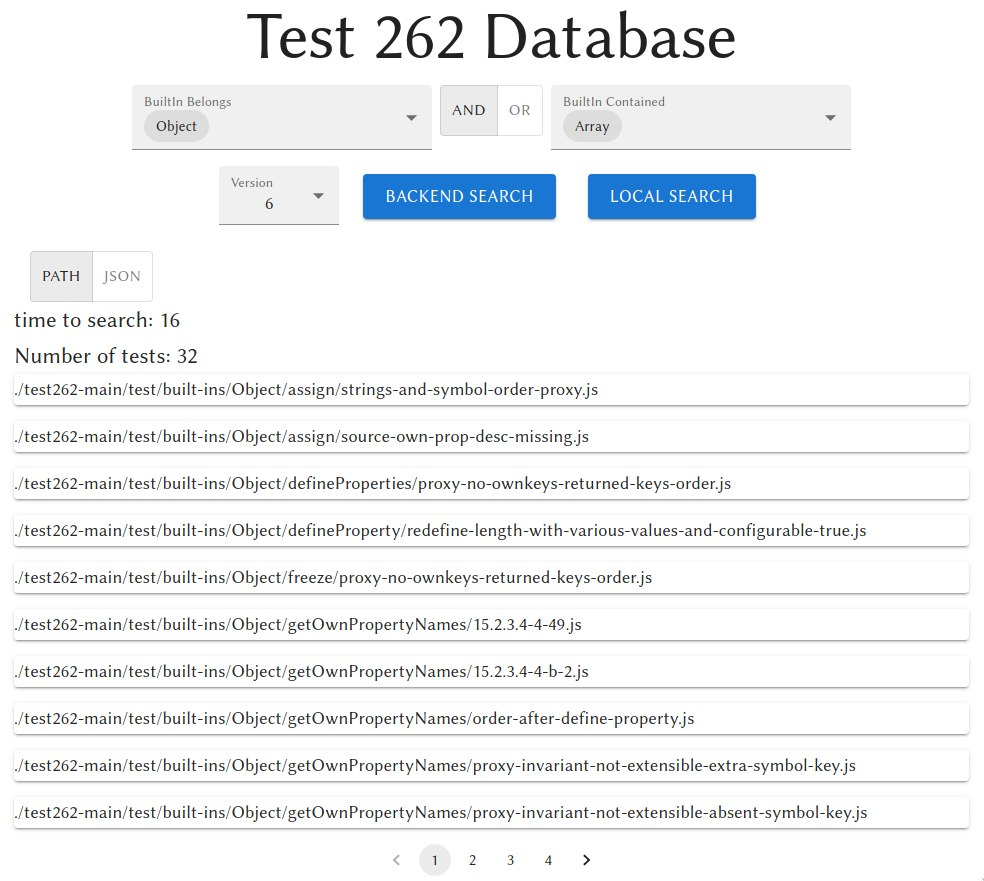
\includegraphics[width=1\textwidth]{images/website.png}
    \caption{\colorbox{orange}{Website} for searching the metadata in construction}
    % QUESTION letra maiuscula na caption
    \label{fig:website}
\end{figure}

\section{Evaluation and Planning}
\label{sec:Evaluation and Planning}
% TODO GANT Diagram
\colorbox{orange}{pedir descricao da teses de uma das primeiras reunioes (iPad)}

\section{Conclusion}
\label{sec:Conclusion}


%
% the environments 'definition', 'lemma', 'proposition', 'corollary',
% 'remark', and 'example' are defined in the LLNCS documentclass as well.
%

%
% ---- Bibliography ----
%
% BibTeX users should specify bibliography style 'splncs04'.
% References will then be sorted and formatted in the correct style.
%
% \bibliographystyle{splncs04}
% \bibliography{mybibliography}
%
\bibliographystyle{splncs04}
\bibliography{references}

\end{document}
